The first thing we want to answer in this paper is about browser features, feature trends, and feature lifespan. We extracted the number of features in each browser version from our dataset. Then by comparing the feature set between different versions we find out how many features are added and removed from each version. We see that Chrome is Adding and removing many more features compared to Firefox. But Firefox removes a bigger portion of its features in each version.

\ali{Add data about feature lifespans}

\begin{figure}[ht]
    \centering
    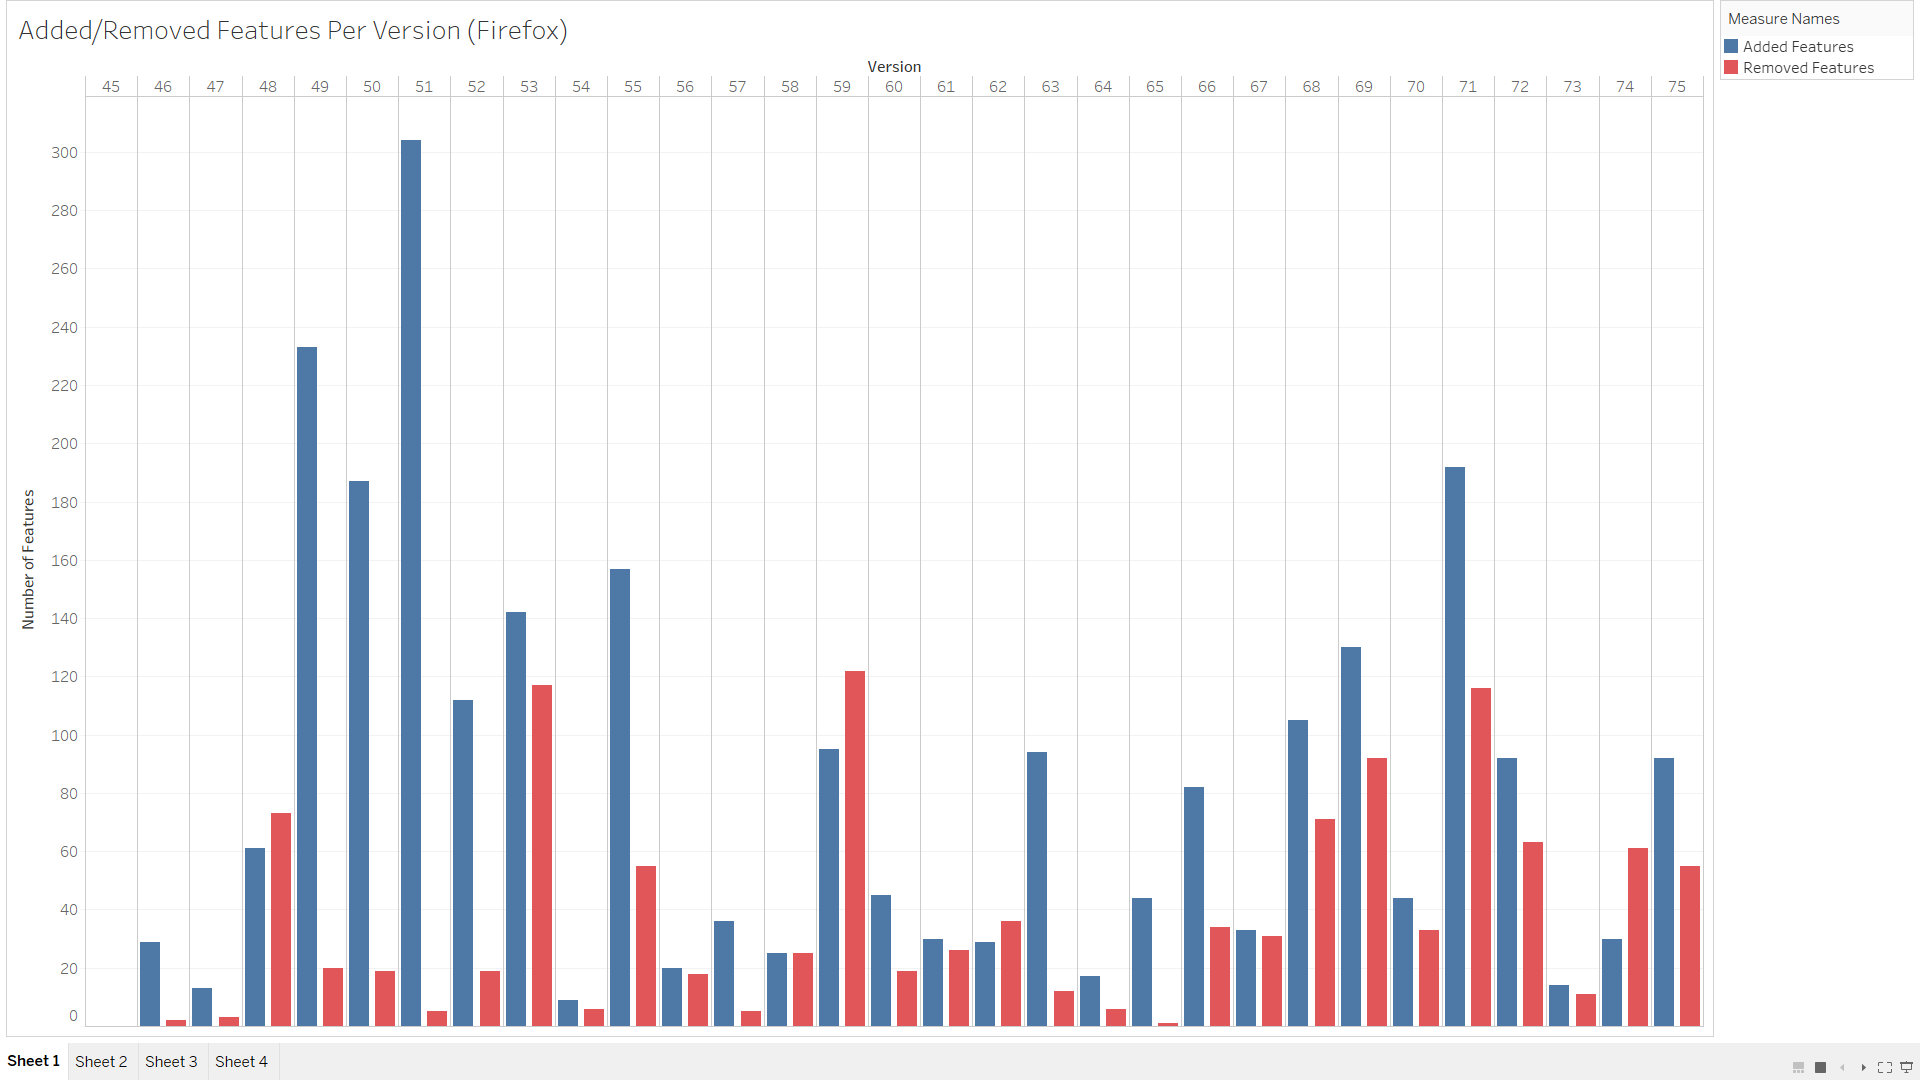
\includegraphics[width=\columnwidth]{figures/Firefox-add-remove.png}
    \caption{Feature Introduction and removal in Firefox. Red bars represent the removed features and the blue bars represent added features.}
    \label{fig:times_bar}
\end{figure}


\begin{figure}[ht]
    \centering
    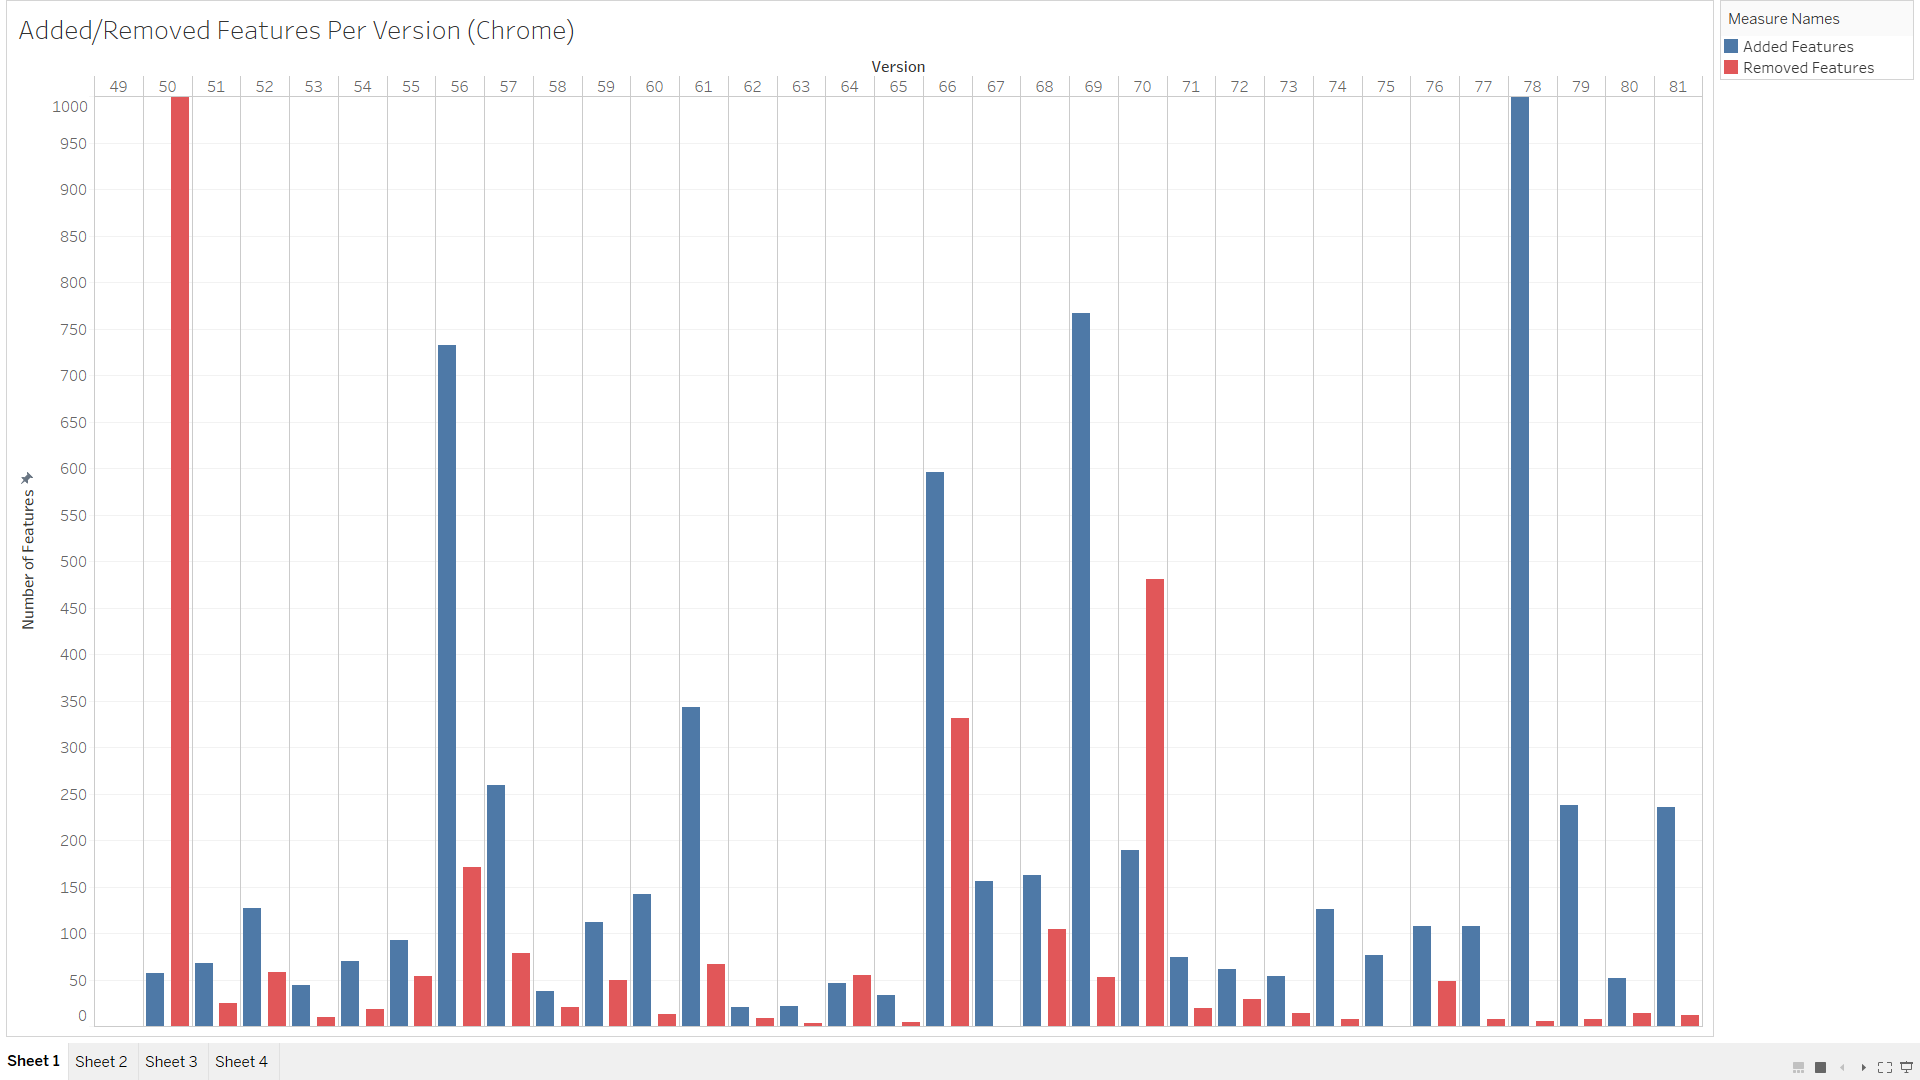
\includegraphics[width=\columnwidth]{figures/Chrome-add-remove.png}
    \caption{Feature Introduction and removal in Chrome. Red bars represent the removed features and the blue bars represent added features.}
    \label{fig:times_bar}
\end{figure}

By using the extracted data for the previous part, we tried to compare feature trends in Chrome and Firefox. We see that Chrome is adding many more features to its browsers comparing to Firefox. Firefox tries to keep the number of its features more steady. They try to remove a bigger portion of their feature set in each version. We cannot say one of them is following the other one in terms of feature introduction and removal.

\begin{figure}[ht]
    \centering
    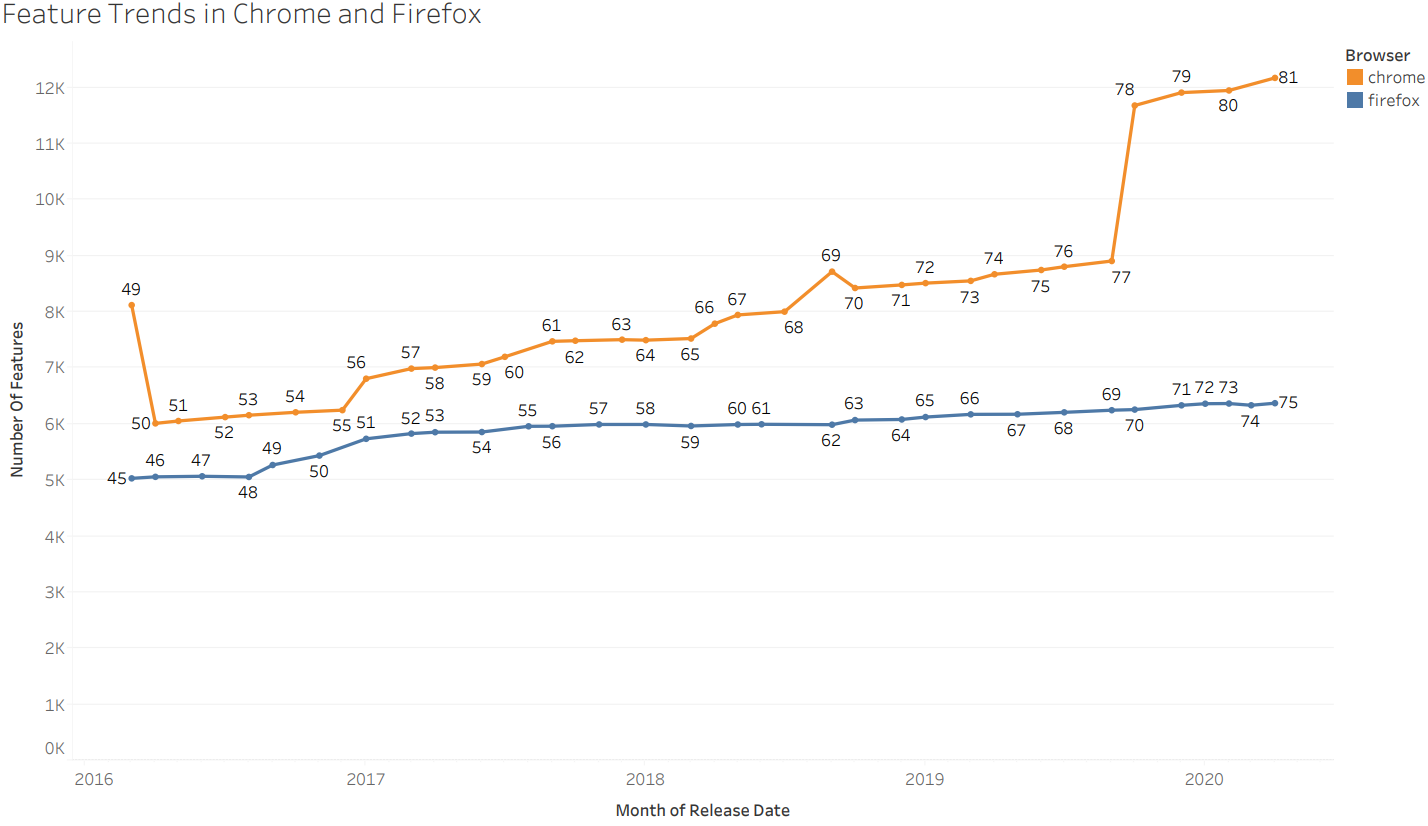
\includegraphics[width=\columnwidth]{figures/Feature-Trends.PNG}
    \caption{Feature trends in Firefox and chrome. The blue line represents the number of features in chrome. The yellow line represents Firefox.\ali{Need to re-scale the chart so the text could be visible}}
    \label{fig:times_bar}
\end{figure}
